\documentclass{article}
\usepackage{geometry}
\usepackage{graphicx}
\usepackage{watermark}
\usepackage[dvipsnames]{xcolor}
\graphicspath{ {./images/} }

\usepackage[hidelinks]{hyperref}
\usepackage{fancyhdr}
\pagestyle{fancy}
\setlength{\headheight}{40pt}
\usepackage{amsmath}
\usepackage{amssymb}
\usepackage{multirow}
\usepackage{placeins}
\usepackage{pdfpages}
\usepackage[export]{adjustbox}

\newcounter{question}
\setcounter{question}{0}
%Que{} per la domanda
\newcommand\Que[1]{
   \leavevmode\par
   \stepcounter{question}
   \noindent
   \thequestion. Q - #1\par}

%Ans[]{} per la risposta, quello che scrivi tra le graffe è in grassetto
\newcommand\Ans[2][]{
    \leavevmode\par\noindent
   {\leftskip25pt
    A - \textbf{#1}#2\par}}

%Spec{} per eventuali spiegazioni della risposta, che finiscono sotto in font più piccolo
\newcommand\Spec[1][]{%
    \medskip\small{#1}}

%\m perchè mi pareva più ordinato rispetto a mettere i dollari ogni 2 secondi
\newcommand{\m}[1]{$#1$}
%\ma per testo matematico da mettere a capo centrato super figo senza sbattersi per il begin center
\newcommand{\mat}[1]{\abovedisplayskip=3pt\begin{gather*}#1\end{gather*}\belowdisplayshortskip=3pt}
%\fa per il "per ogni"
\newcommand{\fa}{~\forall~}
%\EX per il simbolo del valore atteso
\DeclareMathOperator{\EX}{\mathbb{E}}
%per le lettere matematiche fighe
\newcommand{\ml}[1]{\mathbb{#1}}

%per il watermark inutile ma figo nella prima pagina
\thiswatermark{
    \centering
    \put(-370,-690) {
      
\includegraphics[width=1.8\linewidth]{unipdbg}
    }
}

\title{%
Game Theory  Q\&A\\[3ex]
\large{prof. Thomas Marchioro\\
UniPD}}
\author{Giovanni Zago}
\date{a.y. 2023/24}


\begin{document}

\fancyhead{}
\fancyhead[L]{
\includegraphics[height=\headheight]{UnipdLogo}}
\fancyhead[R]{
\includegraphics[height=\headheight]{DEILogo}}
\fancyhead[C]{Gratuitamente avete ricevuto, gratuitamente date\\\scriptsize{\textit{-Mt 10, 8}}}

\fancyfoot{}
\fancyfoot[C]{\scriptsize{For any mistake or suggestion, \href{mailto:giovanni.zago.3@studenti.unipd.it}{contact me}}}
\fancyfoot[R]{\thepage}

\pagenumbering{gobble}

\makeatletter
    \begin{titlepage}
        \begin{center}
            
\includegraphics[width=0.2\linewidth, right]{DEILogo.jpg}\\[20ex]
            {\huge \bfseries  \@title }\\[5ex] 
            {\LARGE  \@author}\\[40ex] 
            {\large \@date}
        \end{center}
    \end{titlepage}

\tableofcontents

\newpage
\pagenumbering{arabic} 

\input{Lectures/Cheatsheet}
\newpage
\section{Introduction, background concepts, decision problems}
\Que{What is a game in game theory?}
\Ans[Game theory]{ is a mathematical framework that allows to model specific type of problems. The problems studied by game theory are called games.}

\Que{What is a game?}
\Ans[A game]{ is a multi-person multi-objective problem.}
\medskip
\small{
\textbf{Multi-person} = There are multiple agents (players) involved in a game

\textbf{Multi-objective} = Players have, in general, different goals

The \textbf{outcome} of a game depends on the choices made by all players

The \textbf{purpose} of game theory is to find the “best choice” for each of them according to their objectives}

\Que{What does it mean for a preference to be rational?}
\Ans[A preference]{ is rational when it's complete and transitive}
\medskip
\small{\textbf{Preference} is a binary relationship $\succeq$ between
elements of \m{A} (set of possible actions)

If \m{a,b \in A, a \succeq b}  means that \m{a} is preferred to \m{b}

A \textbf{preference} is always: reflexive, anti-symmetric
A preference can also be:
\begin{itemize}
    \item \textbf{complete} if \m{\fa a,b \in A} either \m{a \succeq b} or \m{b \succeq a}
    \item \textbf{transitive} if \m{\fa a,b \in A, a \succeq b \wedge b \succeq c \Rightarrow a \succeq c}
\end{itemize}}

\Que{What does it mean for a player to be rational?}
\Ans[A player is rational]{ when he always maximize their utility function, i.e., choose the action that leads to his preferred
outcome. In other words, rational player act for their own good.}

\Que{What are the elements of a decision problem?}
\Ans[A decision problem]{ has three elements: actions, outcomes and preferences.}
\medskip
\small{
\textbf{Action} \m{a} is selected from a set of possible actions \m{A}

Action \m{a} results in a certain \textbf{outcome} (For 1-player problems actions = outcomes)

\textbf{Preferences} describe the relationship between different outcomes (i.e., which one is preferred)}

\Que{How to represent a decision tree?}
\Ans[A decision tree]{ has players on nodes, actions on branches and payoffs on leaves.

\begin{center}
    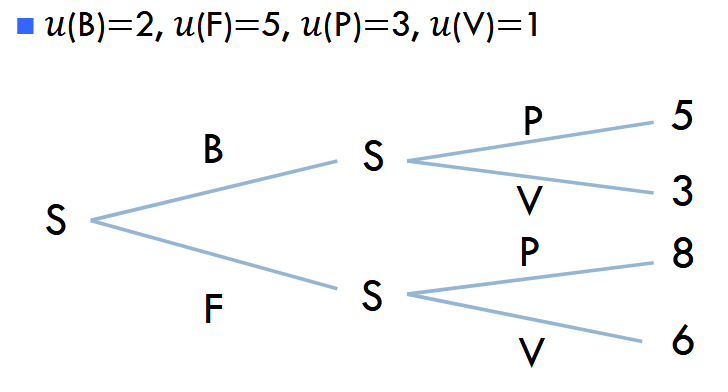
\includegraphics[width=0.5\textwidth]{decTree}
\end{center}}
\newpage
\section{Lotteries, VNM utility theorem, backward induction}

\Que{When is it possible to model preferences between
lotteries using average payoffs?}
\Ans[]{When radmness is involved, i.e. when some events are called as nature ($N$) events, not in the hand of the player.}

\Que{Which utility function can we use to model a risk-
averse player? 1) \m{u(x) = x^2} or 2) \m{u(x) = log(x)}?}
\Ans[2)]{Log funct models risk-averse: he prefers lower results with higher probability.}

\Que{How can we solve a decision problem involving
sequential choices made by both a player and
Nature?}
\Ans[]{Having the decision tree, starting with nodes at the end of the tree, substitute $N$ node with expected utility and player's move with payoff of the best move.}
\Spec{\textbf{Expected utilty} is calculated as probability expected value:

\m{\EX_{x \sim p}[u(x)] = \sum_{k=1}^n p(x_k)\cdot u(x_k)} where $p$ is the payoff and $u$ is the utilty (u don't say)}
\newpage
\section{Static games of complete information, normal-form representation, strictly dominated strategies, IESDS}
\begin{center}
    (No questions in slides)
\end{center}

\Que{When a strategy is called Pareto dominated?}
\Ans[A joint strategy $s$ is Pareto-dominated]{ by another strategy
$s^{'}$ if 
\begin{itemize}
    \item \m{u_i (s^{'}) \geq u_i (s)} for each player $i$
    \item \m{u_i (s^{'}) > u_i (s)} for some player $i$
\end{itemize}
}

\Que{What is IESDS?}
\Ans[IESDS]{ stands for "iterated elimination of strictly
dominated strategies". Since a rational player will never play a Pareto-dominated strategy, with IESDS is possible to delete one Pareto-dominated strategy after the other, in order to get a set of just one strategy or at least an easier rapresentation of the game.}
\newpage
\section{Nash equilibrium, best response, weak dominance, price of anarchy}

\Que{What is a NE}
\Ans[Nash equilibrium ]{is what is played if believes of both players match.}
\Spec{A \textbf{belief} of player $i$ is a possible profile of other player's strategy.

A \textbf{best strategy} is the response of a rational player to a believe. i.e. strategy $s_i \in S_i$ is a BS to moves \m{(s_1,...,s_{i-1},s_{i+1},...,s_n)} if \mat{(s_1,...,s_{i-1},\textcolor{red}{s_i},s_{i+1},...,s_n) \geq (s_1,...,s_{i-1},\textcolor{blue}{s'_{i}},s_{i+1},...,s_n)\\\fa \textcolor{blue}{s'_{i}} \in S_i}}

\Que{Consider NE \m{(s_1,...,s_n)}. Suppose player $i$ replaces the
current strategy $s_i$ with \m{s'_i}. Can this still be a NE?}
\Ans[No.]{ In Nash equilibrium no player can improve his payoff unilaterally.}

\Que{If a strategy is ruled out by IESDS, can it be a NE?}
\Ans[Yes.]{ A joint strategy \m{(s^*_1,...,s^*_n)} in which everyone plays a dominant strategy is a Nash equilibrium.}

\Que{Compute the PoA for the Prisoner’s dilemma using \mat{C(s) = -\sum_j u_j(s)}}
\Ans[]{
\begin{table}[!ht]
    \centering
    \begin{tabular}{cc||c|c}
        \multicolumn{4}{c}{Player B}\\
        \multirow{3}*{\rotatebox{90}{Player A}}
        &    & M     & F     \\ \cline{2-4}
        &M   & -1,-1 & -9,0  \\ \cline{2-4}
        &F   & 0,-9  & -6,-6 \\
    \end{tabular}
    \caption{Prisoners' dilemma}
\end{table}

Worst (and, in this case, unique) NE: MM. Best Pareto: MF or FM. \mat{PoA = \frac{-[-(-1)+(-1)]}{-[(0)+(-6)]} = \frac{2}{6} = \frac{1}{3}}}
\Spec{The price of anarchy (PoA) is the ratio between the social costs in the worst NE $s^*$ and in the best Pareto efficient strategy (i.e.,
social optimum).\mat{PoA = \frac{C (s^{*})}{min_s~C(s)}}}

\Que{Solve this hw.
\begin{figure}[!ht]
    \centering
    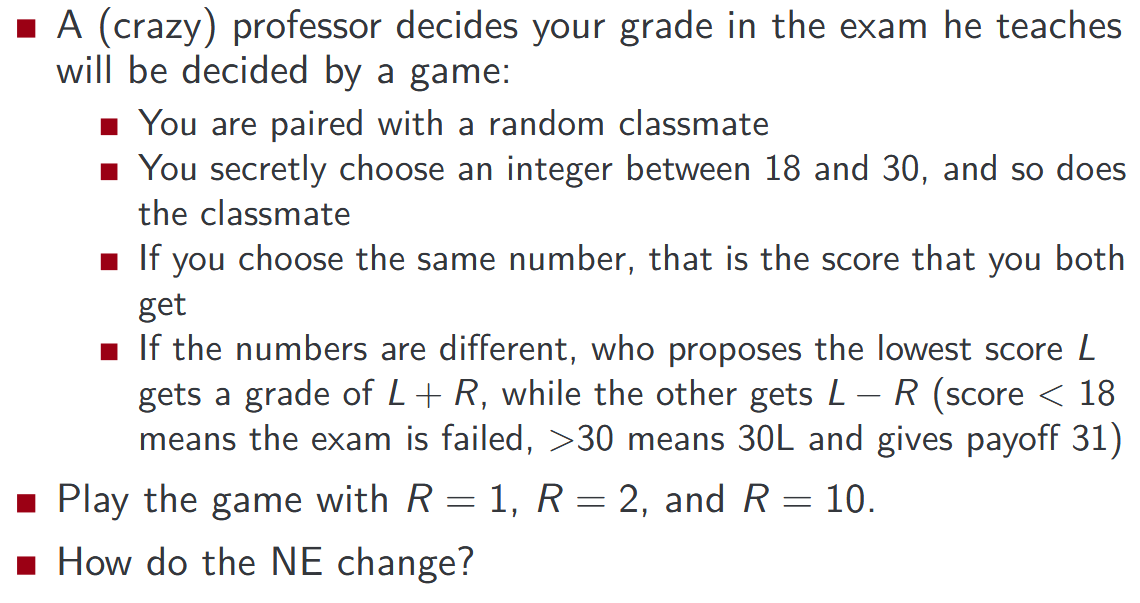
\includegraphics[width=0.5\linewidth]{hw1.png}
\end{figure}
}

\Ans[]{For a generic R
\begin{table}[!ht]
    \centering
    \begin{tabular}{cc|c|c|c|c|c}
        \multicolumn{1}{c}{} & \multicolumn{6}{c}{Player B}\\
        \multirow{6}*{\rotatebox{90}{Player A}}
         & & \textbf{18} & \textbf{19} & \textbf{\dots} & \textbf{29} & \textbf{30}\\ \cline{2-7}
         & \textbf{18} & 18,18 & 18+R,0 & \dots & 18+R,0 & 18+R,0\\ \cline{2-7}
         & \textbf{19} & 0,18+R & 19,19 & \dots & 19+R,21-R & 19+R,19-R\\ \cline{2-7}
         & \textbf{\dots} & \dots & \dots & $\ddots$ & \dots & \dots\\ \cline{2-7}
         & \textbf{29} & 0,18+R & 19-R,19+R & \dots & 29,29 & 29-R,29+R\\ \cline{2-7}
         & \textbf{30} & 0,18+R & 19-R,19+R & \dots & 29-R,29+R & 30,30\\
    \end{tabular}
    \caption{HW1: Strange exam}
\end{table}
\FloatBarrier
For $R = 1$ all couples with same grades are Nash equilibria.

For $R > 1$ the only NE is a Pareto-dominated strategy (i.e., 18,18).
}
\newpage
\section{Exercise on NE, constitutions, electoral systems}
\begin{center}
    (No questions in slides)
\end{center}

\Que{What is a constitution?}
\Ans[Constitution]{, or \textbf{social welfare function}, is a map \mat{f:R(A)^n \longrightarrow R(A)\\(\succeq_1,\dots,\succeq_n) \xrightarrow{f} f(\succeq_1,\dots,\succeq_n)}} which maps a profile of $n$ rational preferences \m{\succeq_{(i)} = (\succeq_i,\dots,\succeq_n)} into a unique rational social preference \m{\succeq = f(\succeq_{(i)})}.

\Que{What are constitution properties?}
\Ans[Properties:]{
\begin{itemize}
    \item \textbf{Independence of Irrelevant Alternatives} (IIA) if for all pairs \m{(\succeq_{(i)}),(\succeq'_{(i)})} \mat{\fa i, \succeq_i|~{a,b} = \fa i, \succeq'_i|~{a,b} \Longrightarrow f(\succeq_{(i)})|~{a,b} = f(\succeq'_{(i)})|~{a,b}} i.e., adding or removing elements to the set of alternatives does not change the output of a constitution for the pair \m{\{a, b\}}
    \item \textbf{Pareto-efficiency}: constitution $f$ is Pareto-efficient if $\fa$ profiles \m{(\succeq_{(i)})}, for all $a,b \in A$ \mat{\fa i, a \succeq_i b \Longrightarrow a \succeq b} where \m{\succeq~= f((\succeq_{(i)})}. i.e., if everyone prefers $a$ over $b$, that also becomes the preference of the constitution
    \item \textbf{Dictatorship} if \m{\exists i} s.t. \mat{a \succeq_i b \Longrightarrow a \succeq b} where \m{\succeq~= f((\succeq_{(i)})}. i.e., if the constitution simply mimics $i$'s preferences.
    \item \textbf{Monotonic} if a single individual ranking higher $a \in A$ never causes $a$ rank lower in the constitution
    \item \textbf{Non-imposition} is satisfied if all rational preferences can be outputs
\end{itemize}}
\Ans[Theorems:]{
\begin{itemize}
    \item Arrow, 1951: there is no constitution $f$ for which all there properties hold at the same time: $f$ is not a dictatorship, $f$ is monotonic, $f$ satisfies IIA and non-imposition
    \item Arrow, 1963 (Arrow's impossibility theorem): if constitution $f$ is Pareto-efficient and satisfies IIA $\Longrightarrow$ $f$ is a dictatorship
\end{itemize}
}

\Que{Game theory and elections}
\Ans[]{
In an election a candidate the beats (by majority) all the others is called the \textbf{Condorcet winner}. If there is no winner, then there is a cycle (i.e., A $>$ B, B $>$ C, C $>$ A) called \textbf{Condorcet cycle}. With more than 3 candidates there can be a winner and a cycle. With preferences sufficiently randomized and a large (\m{n\longrightarrow \infty}) numbers of candidates, Condorcet cycles are sure to occur
\begin{table}[!ht]
    \centering
    \begin{tabular}{|l|l|l|l|l|l|}
    \hline
        voters$\rightarrow$\\choices$\downarrow$ & 3 & 5 & 7 & 9 & $\infty$ \\ \hline
        3 & 5.6\% & 6.9\% & 7.5\% & 7.8\% & 8.8\% \\ \hline
        5 & 16.0\% & 20.0\% & 21.5\% & 23.0\% & 25.1\% \\ \hline
        7 & 23.9\% & 29.9\% & 30.5\% & 34.2\% & 36.9\% \\ \hline
        $\infty$ & 100.0\% & 100.0\% & 100.0\% & 100.0\% & 100.0\% \\ \hline
    \end{tabular}
\end{table}
}
\FloatBarrier
\Que{What electoral methods we have?}
\Ans[]{We have these methods, all with their strengths and weaknesses
\begin{itemize}
    \item \textbf{Plurality voting}: each voter sort candidates in order of personal preference. The candidate with most first places, wins.
    
    With this method, a candidate with a minority high preference (i.e., being in first place by less than 50\% of voters) wins over candidates in lower places by majority (i.e., if A is in first place for 4/10 voters, in last place for others, B is in second place for all voters and other first places are distributed by other candidates, A wins even if B is preferred by the majority over A)
    \item \textbf{Two-phase run-off}: first round voting: select two candidates with highest amount of votes; second round voting: run-off between those candidates.
    
    With this method, a candidate being the "second choice" for a large majority will never be in the second phase, even if he is preferred to the others by majority (i.e. candidate C has few first place votes but it's preferred to A by every B's voter and it's preferred to B by every A's voter. It will not pass to the second phase, even if it's the Condorcet winner)
    \item \textbf{Borda counting}: suppose we have M candidates, each person gave M-1 points to his favourite candidate, M-2 to the second and so on till the last-favourite, who receive 0 points.

    With this method, a strong candidate voted by the majority and being in last position by the others loses against a candidate being mediocre (i.e., A is voted in first place by half voters and last place by the other half. Considering first two position of the other half equally distributed by B and C, A is the Condorcet winner. But B or C will win elections thanks to all the second place points). Borda counting has also an huge issue with dropouts: a single contestant withdrawn can totally change the outcome. {\tiny(examples in slides)}
    \item \textbf{Approval voting}: each voter can give more than one preference, every preference is a vote, the number N of preferences goes from 1 to M, with M the number of candidates (for N=1 we are in plurality voting).

    Depending on N, less favourite candidates has less or more chances to win.
    \item \textbf{Instant run-off}: asking voters to place candidates in order of preferences, only first placed goes counts in order to second round voting. Iteratively, we remove candidates with lowest amount of top preferences, till we get a majority.

    Also in this scenario, a small change (even an increase in preferences) can lead to a different outcome.
\end{itemize}
}
\newpage
\section{NE applications (Duopolies, tragedy of the commons, selfish routing)}
\begin{center}
    To be better understand
\end{center}
\newpage
\section{Mixed strategies, Nash theorem}

\Que{What is a mixed strategy?}
\Ans[A mixed strategy ]{for player $i$ is, in a game \m{G = (S_1,\dots,S_n;u_1,\dots,u_n)} a probability distribution $p_i$ over set $S_i$.

i.e. choosing strategies \m{S_i = (s_i^{(1)},\dots,s_i^{(k)}) with probabilities (p_i(s_i^{(1)}),\dots,p_i(s_i^{(k)}))}}

\Que{What is expected utility?}
\Ans[Expected utility ]{is (as expansion of utility) a real function over \m{\Delta S_1 \times \dots \times \Delta S_n}. For a chosen mixed strategy, payoff can be calculated as a weighted average over $p_i$. \mat{u_i(p_i,\dots,p_n) = \sum_{(s_1,\dots,s_n)\in S}p_1(s_1)\cdots p_n(s_n)\cdot u_i(s_1,\dots,s_n)} with \m{S = S_1 \times \cdots \times S_n}.

Strict and weak dominance are, as always, $>$ or $\geq$. Nash equiibrium is based on expected utility.}

\Que{What is the support of a mixed strategy?}
\Ans[]{Given a mixed strategy $p_i\in \Delta S_i$ we define the support of $p_i$ as \m{supp(p_i) = s_i \in S_i : p_i(s_i) > 0} (if $p_i(s_i) = 1$, $s_i$ is a pure strategy).}

\Que{Nash theorem}
\Ans[]{Every game with finite pure-strategy sets $S_i$ has at least one Nash equilibrium, possibly involving mixed strategies. More formally: for game \m{G = (S_1,\dots,S_n;u_n,\dots,u_n)}, define \mat{BR_i : \Delta S_1 \times \cdots \times \Delta S_{i-1} \times S_{i+1}\longrightarrow 2^{\Delta S_i}} \mat{BR_i(p_{-i}) = {p_i \in \Delta S_i : u_i(p_i,p_{-i}) \text{ is maximized}}}. Then define \m{\textbf{BR}:\Delta S \longrightarrow 2^{\Delta S}} as \mat{\textbf{BR}(p) = BR_1(p_{-1}) \times \cdots \times BR_n (p_{-n})} $p$ is a NE if $p \in BR(p)$}
\newpage
\section{Potential games, congestion games, coordination games; computational complexity of Nash Equilibrium search}

\Que{What is a potential game?}
\Ans[A potential game ]{is a fictitious game that converges to NE. A fictitious game is a game where regrets become actual changes of moves.

Function \m{\Omega : S \xrightarrow{} \mathbb{R}} is an exact potential for $\ml{G}$ if: \mat{\Omega(s'_i,s_{-i}) - \Omega(s_i,s_{-i}) = u_i(s'_i,s_{-i}) - u_i(s_i,s_{-i} = \Delta U_i}

Function \m{\Omega : S \xrightarrow{} \mathbb{R}} is a weighted potential for $\ml{G}$ with weight \m{w = {w_i > 0}} if: \mat{\Omega(s'_i,s_{-i}) - \Omega(s_i,s_{-i}) = w_i \Delta u_i}

Function \m{\Omega : S \xrightarrow{} \mathbb{R}} is an ordinal potential for $\ml{G}$ if: \mat{\Omega(s'_i,s_{-i}) > \Omega(s_i,s_{-i}) \Longleftrightarrow u_i(s'_i,s_{-i}) > u_i(s_i,s_{-i})}}

\Que{Th: Every potential game has (at least) one NE in pure strategies}

\Que{Which types of potential games does exist?}
\Ans[]{Congestion game: a potential game where players choose the "least congest" resource.

Coordination game: models situations where players have incentive to coordinate their actions.

Dummy (or pure-externality) game: game in such that \m{\fa s_{-i}, u_i(s_i,s_{-i}) = u_i(s'_i,s_{-i})}, i.e. players payoff depends only on $s_{-i}$.

\textbf{N.B.} every potential game is a sum of coordination game and dummy game.}

\Que{What is the computational complexity of finding NE?}
\Ans[It's PPAD.]{ NE theorem states that a solution must exist, so it cannot be NP-complete. On the other hand, finding a NE in some case can be very difficult. Let's say (with the nth abuse of notation) that \m{P<PPAD<NP}. Wich means that $PPAD$ is hard till we demonstrate \m{P = NP}. In this class we find the \href{https://math.stackexchange.com/questions/3236049/end-of-the-line-ppad-complexity}{"end-of-line problem"}.}
\newpage
\section{Only for projects. LOL}
\section{Exercise set \#1 (static games of complete information)}

\begin{center}
    See the end of lectures for exercises and solutions.
\end{center}
\newpage
\section{Dynamic games}

\Que{What is a dynamic game?}
\Ans[A dynamic game]{ is a game in which players moves are sequential and not simultaneous.}
\Spec{They can be of \textbf{perfect information} (meaning that every player can do every decision with full awareness) or \textbf{imperfect information} (meaning some decisions are “simultaneous” or Nature moves).

We have two scenarios for the former information:
\begin{itemize}
    \item \textbf{endogenous uncertainty}: information sets contain multiple nodes (simultaneous moves)
    \item \textbf{exogenous uncertainty}: there is a choice of Nature (lotteries)
\end{itemize}}

\Que{How can we represent dynamic games?}
\Ans[]{Graphically, they can be represented as a tree, where each level is a move and each node is the response to a specific opponent' move.
\begin{figure}[!ht]
    \centering
    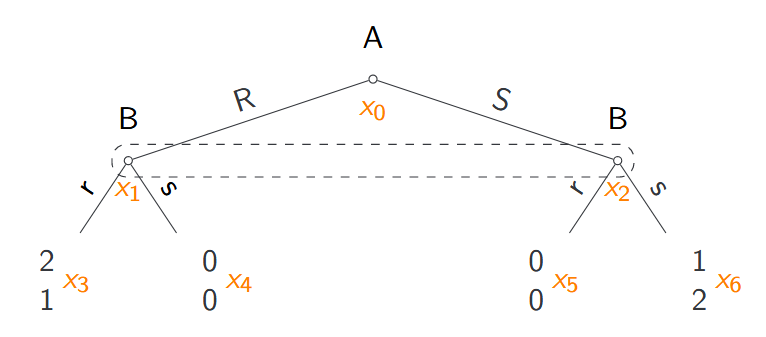
\includegraphics[width=0.5\linewidth]{dynamicTree.png}
\end{figure}
Dotted circle (or just a dotted arch) shows node from the same information set, i.e. the game stage a player can have.

A \textbf{information set} $h_i$ is a mathematical representation of player's possible moves. If $h_i = \{x_j\}$ (i.e. it has just one node), then the node is fully aware of previous moves.}

\Que{How to define a strategy in dynamic games?}
\Ans[]{A strategy in dynamic games need to account for the history of play.

Imagine a two-move game, B has strategy \m{s_B = (a_1, a_2)} where $a_1$ is the response to A playing move 1. If the match is played twice, B has strategy \mat{s_B = (a_1, a_{11}, a_{12}, a_{21}, a_{22})}, where $a_11$ is the answer of A first move, B playing 1 and A answering with 1 (for example, \m{s_b = (1,1,1,1,1)} means B playing 1 no matter what. Instead, \m{s_b = (1,2,1,1,1)} means B playing 2 if A's second move is 1, otherwise playing 1.}
\newpage
\section{Mixed strategies and Nash equilirbia in dynamic games, subgame-perfect Nash equilibria}

\Que{What is the difference between mixed and behavioral strategies? Under what condition are the two concepts equivalent?}
\Ans[Mixed strategies]{ are decided before the game starts; \textbf{behavioral}, on the other hand, are more "realistic" and every move is decided after opponent makes his (more formally: at each information set, select a random move from your set of available moves). They are equivalent under the perfect \textbf{recall assumption}: players do not forget the information they have acquired.}

\Que{How do you find the solution(s) of a sequential game?}
\Ans[By backward induction:]{ starting from the leaf with maximum payoff for the player, replace the parent node with the payoff, repeat until root.
More formally:
\begin{itemize}
    \item Start from the leaves of the tree
    \item Partition them according to their parent node (which is a move of some player $i$)
    \item For each set in the partition, find the leaf $x_j$ with maximum payoff for player $i$
    \item Add the corresponding branch to player $i$’s strategy
    \item Replace the parent node with the payoff of $x_j$
    \item Repeat until the root is reached
\end{itemize}
Solutions can be unique as can be more than one. This way, we find the \textbf{equilibrium path}.}
\Spec[A (proper) \textbf{subgame} $\ml{G'}$ of a game $\ml{G}$ contains a single node of the tree and all of its descendants, with the requirement that
\mat{x_j \in \ml{G'}, x_j \in h_i \hookrightarrow x_k \in \ml{G'} \fa x_k \in h_i}

An \textbf{equilibrium path} is a path that contains all nodes of a NE alont the tree rapresentation of the game.]

\Que{What is a subgame-perfect NE? In which cases is a NE not subgame-perfect?}
\Ans[A subgame-perfect NE (SPE)]{ is the strategy that yield a NE in every subgame. Every SPE is a NE in the parent game and every finite dynamic game has at least one SPE. This means that every sequential game (tic tac toe, chess etc \dots) has a NE.}

\Que{\textbf{Exercise}

\textit{Solution can be found in Lecture13 pdf}

It is the discount sales season, Karen (K) and Lou (L) wants to go shopping. He thinks it is best to wait until the last three days of the discount sales, because prices are cheapest. On day 1, Lou asks Karen (K) to go with him. If Karen says yes (Y), they go shopping and the game ends. If Karen says no (N), Lou can either give up (G) or request (R) again the following day. On day 2, the same happens. On day 3, if K still says N, the game ends as well and does not go into a further day. If in the end K and L do not go shopping, both of their payoffs are 0. If they do, their payoffs are computed as $u_K = d$ and $u_L = 5 - 2d$, respectively, where $d$ is the day in which they go. All of this information about the game is common knowledge among the players.
\begin{enumerate}
    \item Represent the game in its extensive form.
    \item  How many (pure) strategies do K and L have, respectively?
    \item  Find the SPE of this game.
    \item  Find one NE that is not subgame-perfect.
    \item  Represent the game in its normal form.
    \item  Find all the NE of this game (both SPE and non-SPE).
\end{enumerate}
}
\Ans[Solution]{
\begin{enumerate}
    \item 
    \begin{figure}[!ht]
        \centering
        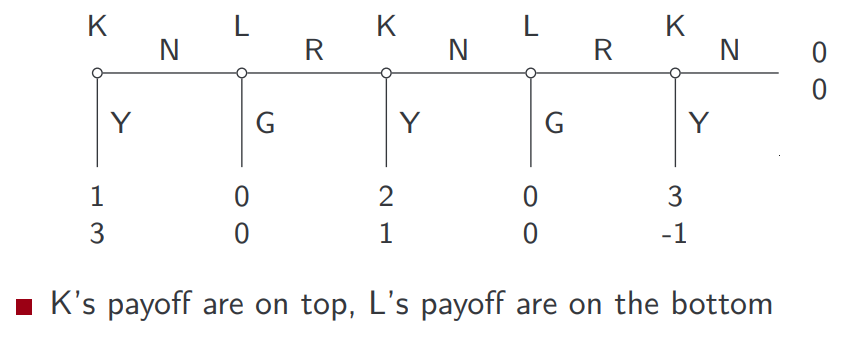
\includegraphics[width=0.5\linewidth]{ex12-1.png}
    \end{figure}

    \item K plays in 3 information sets and has 2 possible actions in each set: $2^3 = 8$ possible strategies. Her strategies are triplets: \m{s_K = (a_0, a_2, a_4), a_j \in {Y, N}}
    
    L plays in 2 information sets has 2 possible actions in each set: $2^2 = 4$ possible strategies. His strategies are triplets: \m{s_L = (a_1, a_3), a_j \in {G, R}}
    \item The SPE can be found via backward induction. On the last day, K prefers Y (payoff 3) to N (payoff 0): $a_4 = Y$. Before that, L prefers G (payoff 0) to R (payoff -1, knowing K’s next choice): $a_3 = G$. Before that, K prefers Y (payoff 1) to N (payoff 0, knowing how the rest of the game will play out): $a_2 = Y$. Only SPE: $s_K = (N, Y , Y )$, $s_L = (R, G)$
    \item Just chose and irrational move on SPE (outside equilibrium path)
    \item Just draw it
    \item Trivial and left to the reader
\end{enumerate}
}
\newpage
\section{Multistage games pt. 1}

\Que{What is a multistage game?}
\Ans[A multistage game ]{is a game which consist in a sequence of smaller games, called \textbf{stages}, where total payoff is the sum of every payoff.

Some games can have independent stages (like partial exam), other can have a discount \textbf{factor} $\delta \in [0,1]$ when stages are far apart in time. If so, the total payoff of player $i$ is \mat{u_i = u_i^{(1)} + \delta u_i^{(2)} + \delta^2 u_i^{(3)} + \dots + \delta^T u_i^{(T)} +} Discount is en exponential function of time $t$. It has to be exponential (not linear) because of time consistency.}
\newpage
\section{Multistage games pt 2, stick-and-carrot strategies}

\Que{What is a strategy in a multistage game?}
\Ans[]{Each player has to specify what to do in the first stage and what to do in subsequent games depending on the outcome of previous games.}

\Que{Theorem for independent stages}
\Ans[]{Suppose \m{s^{(t)} = (s_1^{(1)}, \dots, s_n^{(t)})} is a NE strategy for stage $t$ of multistage game $\ml{G}$; then there is a SPE of $\ml{G}$ with equilibrium path \m{(s_1^{(1)}, \dots, s_n^{(t)})}. In other words, a strategy where each player always plays a NE, is a SPE.}

\Que{Theorem for linked stages 1}
\Ans[]{Every NE $s^*$ of multistage game \m{\ml{G} = (\ml{G}_1, \dots, \ml{G}_T)} requires that a NE is played in the last stage. In other words, in order for a strategy to be a NE, it has to have a NE in the last stage, since players already know all previous outcomes.}

\Que{Theorem for linked stages 2}
\Ans[]{If stage games \m{\ml{G}_1, \dots, \ml{G}_T} has all unique NE, then \m{\ml{G} = (\ml{G}_1, \dots, \ml{G}_T)} has unique SPE. In other words, if every stage has only one NE, this is the equilibrium path.

There is a counter intuitive consequence of these theorems: if the last stage has multiple NE, that enable non-NE strategies to be played in previous stages.}

\Que{What is the meaning of $\delta$?}
\Ans[$\delta$]{ is the measure of how much we care about the future. A larger $\delta$ means we care more about future payoffs.}

\Que{One-stage deviation principle}
\Ans[]{A one stage unimprovable strategy must be optimal. \textit{(proof in Lecture14)}}
\Spec{\textbf{Optimal strategy}: a strategy $s_i$ is optimal for player $i$ i $\fa$ information set $h_i$ there is no way to improve it (more formally: \m{\nexists s'_i / u_i(s'_i|\{h_i\} > u_i(s_i|\{h_i\}}).

\textbf{One-stage unimprovable strategy}: a strategy $s_i$ is one-stage unimprovable if there is no $s'_i$ that differes in one single stage s.t. \m{u_i(s'_i|\{h_i\} > u_i(s_i|\{h_i\}}}

\Que{Exercise 1}
\Ans[]{Consider multistage game $\ml{G}$ = ($\ml{G}_1$, $\ml{G}_2$), with $\ml{G}_1$ being the first stage, and $\ml{G}_2$ being the second (and last) stage:
\begin{itemize}
    \item Is it possible (for some $\ml{G}_1$ and $\ml{G}_2$) to find a SPE for $\ml{G}$ where a non-NE is played in G2?  \textbf{No}
    \item Is it possible (for some $\ml{G}_1$ and  $\ml{G}_2$) to find a NE for $\ml{G}$ where a non-NE is played in G2? \textbf{No}
    \item Is it possible (for some $\ml{G}_1$ and  $\ml{G}_2$) to find a SPE for $\ml{G}$ where a non-NE is played in G1? \textbf{Yes}
    \item Is it possible (for some $\ml{G}_1$ and  $\ml{G}_2$) to find a SPE for $\ml{G}$ where a strictly dominated strategy is played in G1? \textbf{Yes}
    \item What is the minimum number of NE in stage game $\ml{G}_2$ to enable a carrot-and-stick SPE in G? What characteristics should these NE have? \textbf{At least two NE (stick and carrot)}
\end{itemize}
\textit{Answers are mine, so feel free to mail me if they are wrong}
}

\Que{Exercise 2

Ashley and Brook live together. During the winter break they contemplate giving each other a nice gift (G) for Christmas or not (N). They know each other’s preferences so they are able to buy a gift for 10 euros that is worth like 100 euros for the other. They
make this decision independently and without telling each other. After Christmas, they also consider whether to celebrate New Year’s eve downtown (D) or stay home (H).
For the New Year’s eve celebration, they decide independently of each other in a coordination-game fashion. Staying home has utility of $0$ for both. Going downtown has utility of $50$. However, spending New Year’s eve apart from each other has utility of $-100$ for both. The total payoff of the players is the sum of the partial payoffs in each stage with a discount factor of $\delta$ for the second stage.
\begin{enumerate}
    \item Write down the normal form of both stages of the multi-stage game.
    \item Find a trivial subgame-perfect equilibrium of the game where the players just play a Nash equilibrium in all stages, without any strategic connection.
    \item Is there a strategically connected SPE of the whole game where Ashley and Brook give gifts to each other? If so, show the minimum required discount factor value $\delta$min for that to hold.
\end{enumerate}
}
\Ans[]{
\begin{enumerate}
    \item Normal form of stage game
        \begin{table}[!ht]
            \begin{tabular}{c|c|c}
              & G       & N       \\ \hline
            G & 90 90   & -10 100 \\ \hline
            N & 100 -10 & 0 0    
            \end{tabular}
            \quad
            \begin{tabular}{c|c|c}
              & H         & D       \\ \hline
            H & 0 0       & -100 -100\\ \hline
            D & -100 -100 & 50 50    
            \end{tabular}
        \end{table}
        Only NE in Stage 1 is $(N, N)$

        In stage two NE are: $(H, H)$ (stick) and $(D, D)$ (carrot)
    \item Trivial SPE is playing stages independently: $(NHHHH, NHHHH)$ (or with the carrot)
    \item Cooperative SPE: "play G at stage 1. If $(G, G)$ at stage 1, play D, otherwise play H". Sustainable if $u$(cooperative) + $\delta u$(carrot) $\geq u$(unilateral deviant) + $\delta u$(stick) \m{\longrightarrow 90 + 50\delta \geq 100 + 0\delta \longrightarrow \delta \geq \frac{1}{5}}
\end{enumerate}
}
\newpage
\section{Repeated games, grim trigger, tit for tat, Friedman theorem}

\Que{What is a repeated game?}
\Ans[A repeated game $\ml{G}(T, \delta)$]{ is a dynamic game where a static game $\ml{G}$ is played as a stage game for $t$ times with discount $\delta$. We distinguish between:
\begin{itemize}
    \item finitely repeated games ($T = 1, 2, \dots < \infty$);
    \item infinitely repeated games ($T = \infty$). Here we must have $\delta < 1$, otherwise payoff will diverge.
\end{itemize}}

\Que{Theorems}
\Ans[]{
\begin{enumerate}
    \item The outcome of the last stage is a NE
    \item If stage game $\ml{G}$ only has NE $p^*$, then $\ml{G}(T, \delta)$ has a unique subgame-perfect equilibrium, where every player play $p^*$ in every stage (boring)
\end{enumerate}
}

\Que{Cooperation in finitely repeated games}
\Ans[Cooperation ]{is usually incentived in repeated games but in the last stage, which is played "egoistically". As for multistage games, cooperation is possible if there are multiple NE.}

\Que{Infinitely repeated game}
\Ans[]{Since these games has no last stage, there could be a SPE of $\ml{G}(\infty, \delta)$ in which no stage outcome is a NE of $\ml{G}$.

We call a \textbf{grim trigger strategy} (GrT) a strategy where: start playing M at stage 1, at stage $t > 1$, play M only if outcome of all $t-1$ previous stages was $(M,m)$, otherwise play F.\\With $\delta = 1 - \epsilon$, joint strategy "both play GrT" is a SPE.}

\Que{How can we show that a strategy is a NE in overall game?}
\Ans[]{We only need to compare who options:
\begin{itemize}
    \item Cooperate and keep playing the chosen strategy (payoff $p^*$) forever (\m{u_T = p^* + \delta p^* + \delta^2 p^* + \dots = \frac{p^*}{1-\delta}})
    \item Defect at stage 1 and keep playing other option (payoff $p$) forever (\m{u_T = p + \delta p + \delta^2 p + \dots = p^* + \frac{p \delta}{1-\delta}})
\end{itemize}
In order to find minimum $\delta$ s.t. cooperation is best choice, solve \mat{\frac{p^*}{1-\delta} \geq p + \frac{p \delta}{1-\delta}}
}

\Que{Friedman theorem (a.k.a. "folk theorem")}
\Ans[Theorem]{ Let $\ml{G}$ be a finite static game of complete information. Let $(e_1, e_2, \dots, e_n)$ be the payoffs of a NE of $\ml{G}$ and $(x_1, x_2, \dots, x_n)$ be a feasible payoffs for $\ml{G}$. Suppose $\fa$ NE and $\fa, x_j > e_j$. Then, for $\delta$ close enough to 1, $\ml{G}(\infty, \delta)$ has a SPE with payoffs $(x_1, x_2, \dots, x_j)$.
\begin{figure}[!ht]
    \centering
    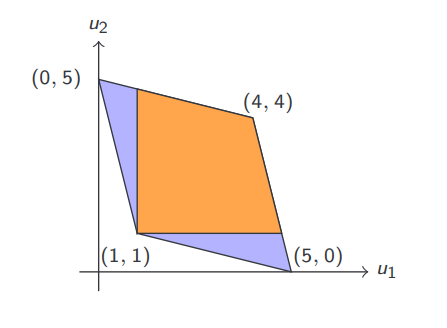
\includegraphics[width=0.3\linewidth]{Friedman.png}
\end{figure}
}
\Spec{A \textbf{feasible payoff} for game $\ml{G}$ is any convex combination \mat{\alpha u(s_1) + \alpha u(s_2) + \dots + \alpha_L(s_L), \text{with} \sum_{i=1}^L\alpha_i=1} of pure-strategy payoffs ($L = |S_1| \cdot |S_2| \dotsm |S_n|$ total numbers of pure strategy)
\begin{figure}[!ht]
    \centering
    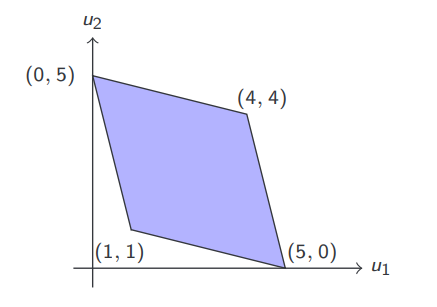
\includegraphics[width=0.3\linewidth]{feasiblePayoff.png}
\end{figure}
}

\Que{Tit for tat (TFT)}
\Ans[TFT ]{is a replacement of GrT where "at stage $t$, play what the other player chose at stage $t-1$", it's a way to avoid keep punishment forever. It has immediately punish deviation but forgiveness after 1-step.

Keep doing TFT forever is called "death spiral" and it's not a NE. generally, NE achieved by TFT is not subgame-perfect.}

\Que{Exercise 1

Consider $\ml{G}$:
\begin{table}[!ht]
\centering
\begin{tabular}{lccc}
& & \multicolumn{2}{c}{Player B} \\
\multirow{3}{*}{\rotatebox{90}{Player A}} & & g & w \\ \cline{3-4} 
& \multicolumn{1}{c|}{G} & \multicolumn{1}{c|}{5, 3} & \multicolumn{1}{c|}{0, 4} \\ \cline{3-4} 
& \multicolumn{1}{c|}{N} & \multicolumn{1}{c|}{6, 0} & \multicolumn{1}{c|}{1,1}  \\ \cline{3-4} 
\end{tabular}
\end{table}
\begin{enumerate}
    \item Is it possible to find a SPE for $\ml{G}$(4) that involves playing (G,g) at each stage?
    \item Is it possible to find a NE for $\ml{G}$($\infty$) where (G,g) is played at each stage using a grim-trigger strategy? If so, for what $\delta$? Is that a SPE?
    \item Is it possible to find a NE for $\ml{G}$($\infty$) where (G,g) is played at each stage using a tit-for-tat strategy? If so, for what $\delta$? Is that a SPE?
\end{enumerate}}
\Ans[]{
TODO:
}

\Que{Exercise 2

Carl (C) and Diana (D) are two university students. Every night they go to the department library, but they do not coordinate or plan any action together. Upon their arrival, they independently decide whether to: (S) study or (M) watch some movies on their laptop. If they both study, they both
get utility 10. The individual benefit from watching a movie is instead 15 for C and 18 for D. However, if they both choose M, their individual benefit is halved (since they have half the
connection speed). Also, trying studying while somebody else is playing a movie breaks the concentration, so $u_C(S,M) = u_D(M,S)$ = 0. Call $\ml{G}$ this game, and consider it in a repeated version $\ml{G}$(T). Individual payoffs are summed with discount factor $\delta$.
\begin{enumerate}
    \item Find the Nash equilibria of $\ml{G}$(3), for $\delta$ = 1
    \item What values of $\delta$ allow for sustaining a Nash equilibrium of $\ml{G}$($\infty$) via a “Grim Trigger” strategy where each player ends up in always choosing S?
    \item Consider an extended game where a punishment strategy P is also available to both players. When either player P, payoffs are -10 for both players (that would correspond, e.g., to do something really stupid in the library and get the library permanently closed). Call this game $\ml{G}$' . If you see a SPE of $\ml{G}$'(2) where players may play S, state at which round do they play it, and what value of $\delta$ do you need to obtain it.
\end{enumerate}}
\Ans[]{
TODO:
}
\newpage
\section{Repeated games (part 2), zero-sum games, minimax theorem}

\Que{What are maximin and minmax?}
\Ans[Maximin and minmax]{ are strategis s.t.:
\begin{itemize}
    \item \textbf{Maximin} \mat{w_i = \max_{s_i \in S_i} \min_{s_{-1} \in S_{-i}} u_i(s_i, s_{-i})} In other words, it's about finding a security strategy (a conservative approach in order for $i$ to achieve the highest payoff against $-i$ the worst move) $s^*_i = \arg\max_{s_i} f_i(s_i)$ with \mat{f_i:S_i\xrightarrow{}\ml{R}, f_i(s_i) = \min_{s_{-i} \in S_{-i}}u_i(s_i,s_{-i})} Then evaluate $w_i = f_i(s^*_i)$ 
    \item \textbf{Minimax} \mat{z_i = \min_{s_{-1} \in S_{-i}} \max_{s_i \in S_i} u_i(s_i, s_{-i})} In other words, it's about finding a strategy for $i$ to calculate the minimum payoff against $-i$ move: $s^*_{-i} = \arg\min_{s_i} F_i(s_i)$ with \mat{F_i:S_i\xrightarrow{}\ml{R}, F_i(s_i) = \max_{s_i\in S_i} u_i(s_i,s_{-i})} Then evaluate $z_i = F_i(s^*_{-i})$
\end{itemize}
}
\Spec{\textbf{Example}

\begin{table}[!ht]
\centering
\begin{tabular}{lc|c|c|c|c}
& & \multicolumn{3}{c}{Player B}       \\
\multirow{3}{*}{\rotatebox{90}{Player A}} & & L & C & R & $f_A(\min)$\\ \cline{3-5} 
& T & 5, - & 3, - & 4, - & 3           \\ \cline{3-5} 
& D & 2, - & 6, - &  1, - & 1          \\ \cline{3-5}
& $F_A(\max)$ & 5 & 6 & 4               \\
\end{tabular}
\end{table}
Maxmin of A : 3

Minimax of A: 4}

\Que{Consequences of maximin and minimax}
\Ans[]{We can prove that, if joint strategy is a NE \mat{maxmin_i \leq minmax_i \leq u_i(NE)}If joint strategy is not a NE then just first disequation}

\Que{Zero-sum games}
\Ans[Zero sum game ]{has the property \mat{u_i(s) = -u_i(s)} (in every cell you have $x,-x$)}

\Que{Adversarial games}
\Ans[Adversarial games ]{are a more general type of games where two players are adversaries and have utilities s.t. \mat{u_i\uparrow \Longleftrightarrow u_{-i}\downarrow} Many adversarial game can be framed as a zero-sum game with this trick: \m{u_A = \text{points}_A - \text{points}_B} and \m{u_B = -\text{points}_A}}

\Que{Theorem}
\Ans[For zero-sum game]{
Let $\ml{G}$ be a zero-sum game with finite number of strategies. Then,
\begin{enumerate}
    \item $\ml{G}$ has a pure NE $\Longleftrightarrow maximin_i = minimax_i$ for each player $i$
    \item All NE yield the same payoffs $(minimax_i ,-minimax_i)$
    \item In all NE, every player is playing a security strategy
\end{enumerate}
}

\Que{Consider a generic game $\ml{G}$
\begin{itemize}
    \item Is $maximin_i$ always equal to $minimax_i$ for each player $i$?
    \item Is $maximin^p_i$ always equal to $minimax^p_i$ for each player $i$?
    \item If $maximin_i = minimax_i$ for each player $i$, does that mean that the game has a pure NE? Does your answer change if $\ml{G}$ is zero-sum?
    \item If $\ml{G}$ is a zero-sum game between $i$ and $-i$, is there a relationship between the minimax of $i$ and the maximin $-i$?
\end{itemize}
}
\Ans[]{TODO:}

\Que{What is the value of a zero-sum game? Does it always exist if the game has infinitely many strategies?}
\Ans[]{TODO:}
\newpage
\section{Stackelberg games, dynamic bargaining}

\Que{Stackelberg game}
\Ans[A Stackelberg game ]{is a sequential version of a static game. Players move one after the other (first the leader, than he follower). Result, which can be obtained via backward induction, is called a Stackelberg equilibrium.}

\Que{How to find Stackelberg equilibrium}
\Ans[]{First find best options of the follower, then among these options, the best one for the leader. In case of a tie, we can have
\begin{itemize}
    \item generous follower
    \item generous leader
\end{itemize}
}

\Que{Stackelberg game consequences}
\Ans[]{
\begin{itemize}
    \item leader payoff in Stackelberg equilibrium $\geq$ payoff in NE of the static game
    \item follower payoff, in general, $\geq$ minimax
\end{itemize}
In a rational game, follower knows leader's move, but leader has a full knowledge of the game: can anticipate follower's move.
}

\Que{Dynamic bargain}
\Ans[Bargain ]{means negotiation of resources. (It's a game of negotiation).

Assume two players get to split a given amount of resources, we can use \textbf{dynamic bargaining} where players switch proposer/responder at any stage. If they disagree at any stage till stage $T$, they both get payoff 0. If they agre at stage $0 < t < T$ they get a discount $\delta^{t-1}$.

Is the deadline is $T=1$ the game is called \textbf{Ultimatum game}.}

\Que{SPE of dynamic bargain}
\Ans[Proposition: ]{Any SPE of the dynamic bargaining game must have the players reaching an agreement in the first round
\begin{itemize}
    \item Simply a consequence of backward induction
    \item Iterating the game: (i) wastes reward because of the discount; (ii) sends the players to another round of proposer-responder, which rational players want to avoid
\end{itemize}

For $T\xrightarrow{}\infty$ we have \mat{u_1 = \frac{1}{1+\delta}} \mat{u_2 = \frac{\delta}{1+\delta}}}
\newpage
\section{Bayesian games}
\Que{Bayesian games}
\Ans[Bayesian games]{ are games of incomplete information, where some players do not have complete knowledge on the other players' utility. Bayesian games have the following assumptions:
\begin{itemize}
    \item Each player i has a set of possible types $T_I=\{\text{type 1},...,\}$
    \item The type of each player $t_1,...,t_n$ is determined by Nature's move at the beginning of the game.
    \item Each player knows only his/her type
    \item Other player's type is unknown
\end{itemize}}
\Que{Preliminary Nature's move}
\Ans[]{Bayesian game scan be seen as a weird kind of dynamic games that is played as follows: Nature draws the type vector $(t_1,..,t_n)$ among all the possible combination of players' types; Nature reveals type $t_i$ only to player i; player choose their action; Final payoffs are computed.}
\Que{Beliefs in Bayesian games}
\Ans[]{To find best responses player create beliefs about these types under the assumption that players do not precisely know the types of their opponents but they have an estimate of those. In other words, they know the probability distribution of the opponents' types. This is called the common prior assumption.}
\Que{Bayesian entry game}
\Ans[]{We have an incumbent (player 1) and and outsider (Player 2). The outsider decides whether to enter the market (E) or stay out (O). The incumbent decides whether to accept the outsider (A) or fight (F). The incumbent could be of two types: reasonable or crazy (in the first case it does not like to fight, in the latter it does). The incumbent knows its type, the outsider estimates reasonable/crazy with probabilities (p,1-p).}
\Que{Normal form of Bayesian games}
\Ans[]{The normal form of Bayesian games can be inferred from the extensive form as we did in dynamic games.}
\Que{Strategies in Bayesian games}
\Ans[]{A strategy specifies what the player does for each type. In the entry game: Player one has two strategies $\{O,E\}$, while player 2 has four strategies: $\{AA,AF,FA,FF\}$. For example if 2 plays AF it means play A if reasonable or play F if crazy.}
\Que{Example to understand the normal form:}
\includepdf[pages=16-23,nup=1x2,landscape=false]{Appendix/Lecture18.pdf}
\Que{Bayesian game: definition}
\Ans[]{It is described as follows:
\begin{itemize}
    \item Set of players $\{1,..,n\}$
    \item Strategy sets $S_1,..,S_n$
    \item Utility functions $u_i:\S_1\times ...\times S_n\rightarrow \mathbb{R}$(for i=1,...,n)
    \item \textbf{Type space} of each player $T_i$
    \item \textbf{Type-dependent utilities:} define $u_i(a_1,...,a_n,t_i)$ for each $t_i\in T_i$
    \item \textbf{Beliefs about players types: }a probability distribution $\phi_i$ defined over types for each player
\end{itemize}}
\Que{Static Bayesian game}
\Ans[]{Consider a static Bayesian game: n players, each player's strategy is just an action:
\begin{itemize}
    \item Player i's type is $t_i\in T_i$, chosen by Nature for each player from 1 to n through the joint prior probability distribution $\phi(t_1,...,t_n)$ where $\phi:T_1\times ...\times T_n\rightarrow[0,1]$
    \item Player i knows his private values of his/her utility function $u_i(a_1,...,a_n,t_i)$
\end{itemize}}
\Que{Type of a player}
\Ans[]{Suppose i can have two different payoff functions $u_{i,A}(a_i,a_{-i})$ and $u_{i,B}(a_I,a_{-i})$. We represent this by setting a type space $T_i=\{t_A,t_B\}$ and imposing $u_{i,j}(a_i,a_{-i})=u_i(a_i,a_{-i},t_j)$.\\
Types can be correlated; they are independent if
\[
\phi(t_1,...,t_n)=\phi(t_1)...\phi(t_n)
\]}
\newpage
\section{Bayesian Nash equilibria, signaling.}
\Que{Static Bayesian game}
\Ans[A static Bayesian game]{ needs a set of player $\mathcal{N}=\{1,...,n\}$, action space $A_1,...,A_n$(pure strategy sets), type space $T_i$(for i=1,...,n), beliefs (on types) $\phi_1,...,\phi_n$, time-dependent payoffs $u_i(a_1,...,a_n,t_i)$.
\[
\mathbb{G}(\mathcal{N};A_1,...,A_n;T_1,...,T_n;\phi_1,...,\phi_n;u_1,...,u_n)
\]
A \textbf{pure strategy} for i can be seen as a map $s_i:T_i\rightarrow A_i$,i.e., it tells what i plays as his/her type is known. A \textbf{Mixed strategy} for i is a probability distribution over pure strategies.}
\Que{Strategies of Bayesian games}
\Ans[]{We can think of a general strategy as being defined before the type of i is even set. Player i decides a strategy $s_i: T_I\rightarrow A_i$, then if their type is $t_i\in T_i$, they will play $s_i(t_i)$. It allows other players to create beliefs over the strategy of a player who can be of different types}
\Que{Bayesian Nash Equilibrium}
\Ans[A Bayesian Nash Equilibrium ]{is a Nash equilibrium in Bayesian games. In $\mathbb{G}(\mathcal{N};A_1,...,A_n;T_1,...,T_n;\phi_1,...,\phi_n;u_1,...,u_n)$, joint strategy $s^{*}=(s_1^{*},...,s_n^{*})$ is a Bayesian Nash Equilibrium is, for each player i and type $t_i\in T_i, s_i^{*}$ maximizes the expected payoff against $s^{*}_{-i}$:
\[
s_i^{*}=\arg\max_{s_i\in S_i}\sum_{t_{-i}}u_i(s_i,s_{-i}^{*}(t_{-i}),t_i)\phi(t_{-i})
\]
that is the same as:
\[
    \mathbb{E}[u_i(s_i^*,s_{-i}^*(t_{-i}),t_i)|t_{-i}]\geq \mathbb{E}[u_i(s_i,s_{-i}^*(t_{-i}),t_i)|t_{-i}]
\]
Look at slides for some examples}
\newpage
\section{Dynamic Bayesian games, perfect Bayesian equilibrium, signaling games.}
\Que{Bayesian equilibrium path}
\Ans[]{If we have a Bayesian NE $s^{*}=(s_1^{*},...,s_n^{*})$, we say that an information set is \textbf{"on" the equilibrium path} if, given the distribution $\phi$ of types, it is reached with probability $>0$}
\Que{System of beliefs}
\Ans[A system of beliefs $\mu$]{ is a probability distribution over decision nodes for every information set. In other words, it is an estimate of being at a specific node, given an information set. It is a conditional probability $\mathbb{P}(\text{node}|\text{information set})$}
\Que{Perfect Bayesian Equilibrium}
\Ans[A perfect Bayesian equilibrium (PBE)]{is a pair $(s^{*},\mu)$, where $s^{*}$ is a Bayesian equilibrium and $\mu$ is a system of beliefs satisfying the following:
\begin{itemize}
    \item Players must have a system of beliefs
    \item On the equilibrium path they must follow Bayes' rule on conditional probabilities
    \item Off the equilibrium path: arbitrary
    \item Given their beliefs, players are sequentially rational: i.e., they play a best response to their belief
\end{itemize}}
\Que{How do you determine sustainable beliefs values $\mu(x_i)$ for nodes that are on the Bayesian equilibrium path?}
\Ans[]{Apply the Bayesian rule to the node}
\Que{What values can $\mu(x_i)$ have if $x_i$ is off the equilibrium path?}
\Ans[]{}
\Que{Signaling games}
\Ans[A signaling game]{ is a 2-player dynamic Bayesian game, where 1 is the first to move and 2 is the second to move. 1's type is chosen among many possible types, 2 has only one type. 2's beliefs are updated after 1's move.}
\begin{figure}[!ht]
    \centering
    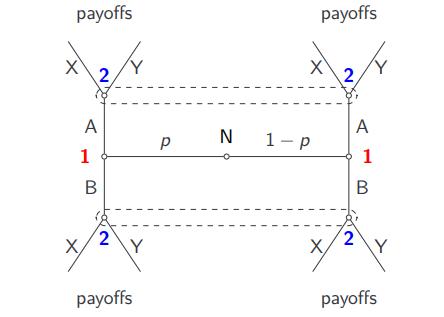
\includegraphics[width=0.5\linewidth]{butt}
    \caption{Representation of the signaling game(butterfly diagram)}
\end{figure}
\Que{Equilibria of signaling games}
\Ans[]{We have 3 kind of equilibria:\begin{itemize}
    \item \textbf{Separating equilibria:} each type of 1 chooses a different action; thus revealing the type to 2
    \item \textbf{Pooling equilibria:} all types of 1 choose the same action; thus, 2 gets no signal about 1's type
    \item \textbf{Intermediate cases:} 1's action does not fully define 1's type, but still provides some information
\end{itemize}}
\Que{Example on butterfly games}
\includepdf[pages=33-52,nup=1x2,landscape=false]{Appendix/Lecture20.pdf}
\Ans[]{Apply the Bayesian rule to the node}
\Que{\textbf{SA1:} consider a dynamic Bayesian game where player 1 moves first and player 2 moves second. Player 1 has three available moves (A,B,C) and only one possible type; player 2 has two available moves (J,K) and two possible types.\begin{itemize}
    \item Draw the game in extensive form (without payoffs)
    \item How many moves specify one strategy of player 1? Why?
    \item How many moves specify one strategy of player 2? Why?
    \item Is SPE enough to characterize the equilibria of the game? Or do you need PBE?
\end{itemize}}
\Que{\textbf{SA2:} Consider a dynamic Bayesian game where player 1 moves first and player 2 moves second. Player 1 has two available moves (C,D) and two possible types $(t_L ,t_R)$ with prior (p,1-p); player 2 has only one type and moves (M,N)
\begin{itemize}
    \item Draw the game in extensive form (without payoffs)
    \item How many moves specify one strategy of player 1? Why?
    \item How many moves specify one strategy of player 2? Why?
    \item Is SPE enough to characterize the equilibria of the game (i.e., to determine wheter a BNE is sequentially rational)? Or do you need PBE?
\end{itemize}}
\Que{\textbf{SA3:} Consider a dynamic Bayesian game where player 1 moves first and player 2 moves second. Player 1 has two available moves (C,D) and two possible types $(t_L ,t_R)$ with prior (p,1-p); player 2 has only one type and moves (M,N)\begin{itemize}
    \item Let $h_D$ be the information set where player 2 moves after observing move D by player 1: what are 2's beliefs values $\mu$ in each node of $h_D$ assuming separating strategy DC for 1?
    \item What are 2's belief values $\mu$ in each node of $h_D$ assuming pooling strategy DD for 1?
    \item What are 2's belief value $\mu$ in each node of $h_D$ assuming pooling strategy CC for 1?
\end{itemize}}

\newpage
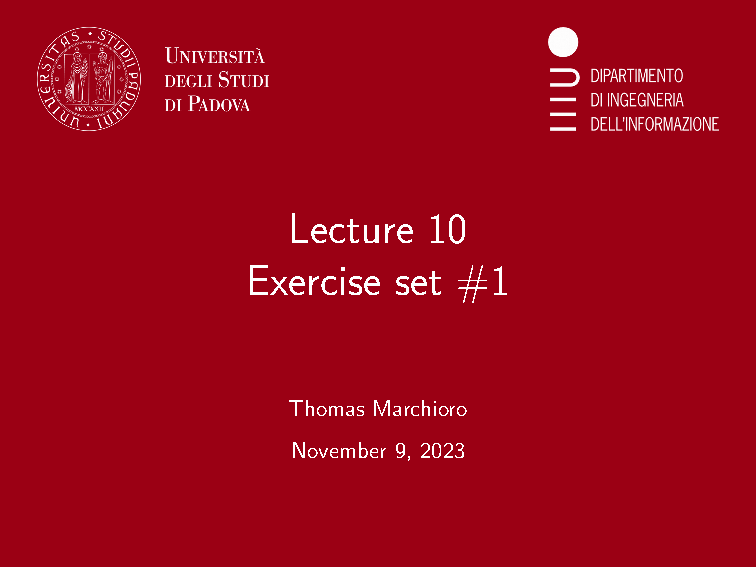
\includepdf[pages=-,nup=1x2,landscape=false]{Appendix/Lecture10.pdf}
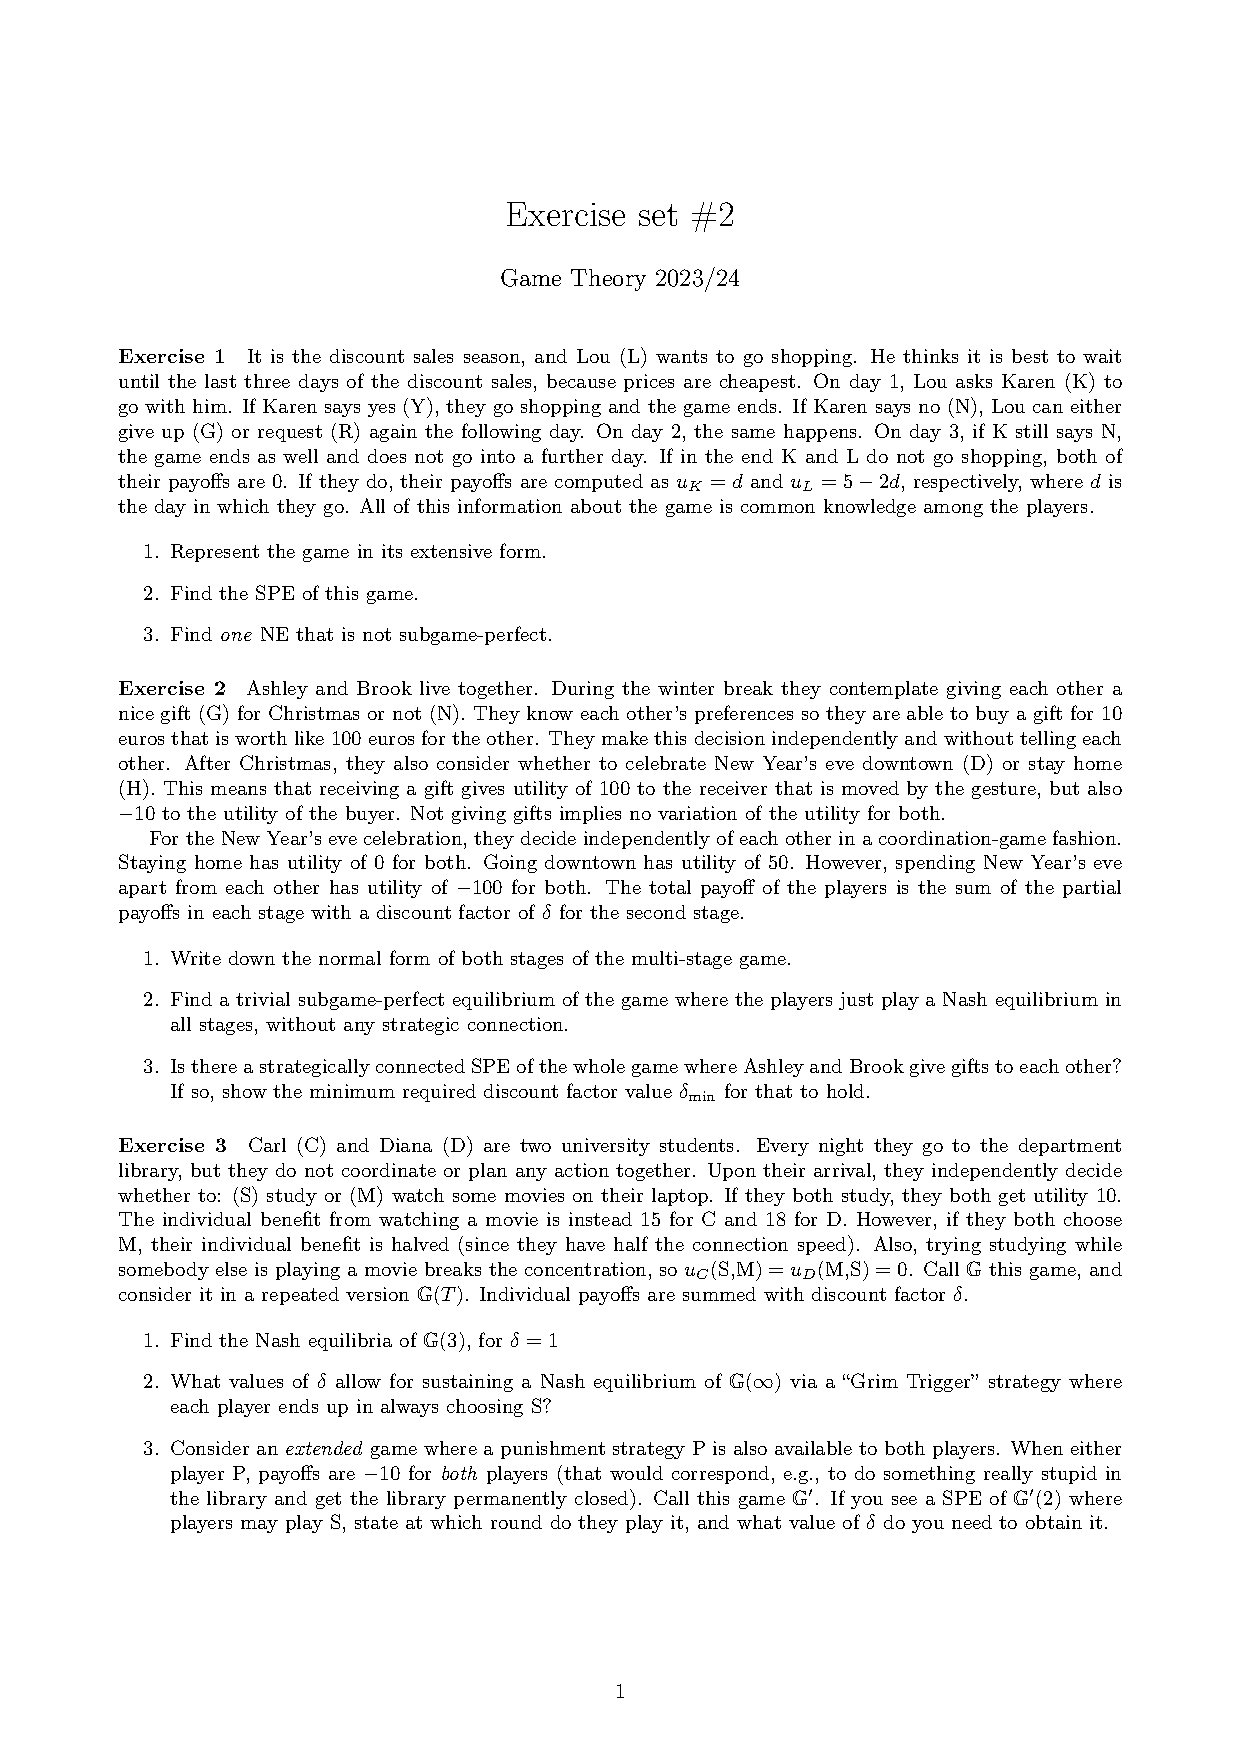
\includepdf[pages=-]{Appendix/Exercise2.pdf}
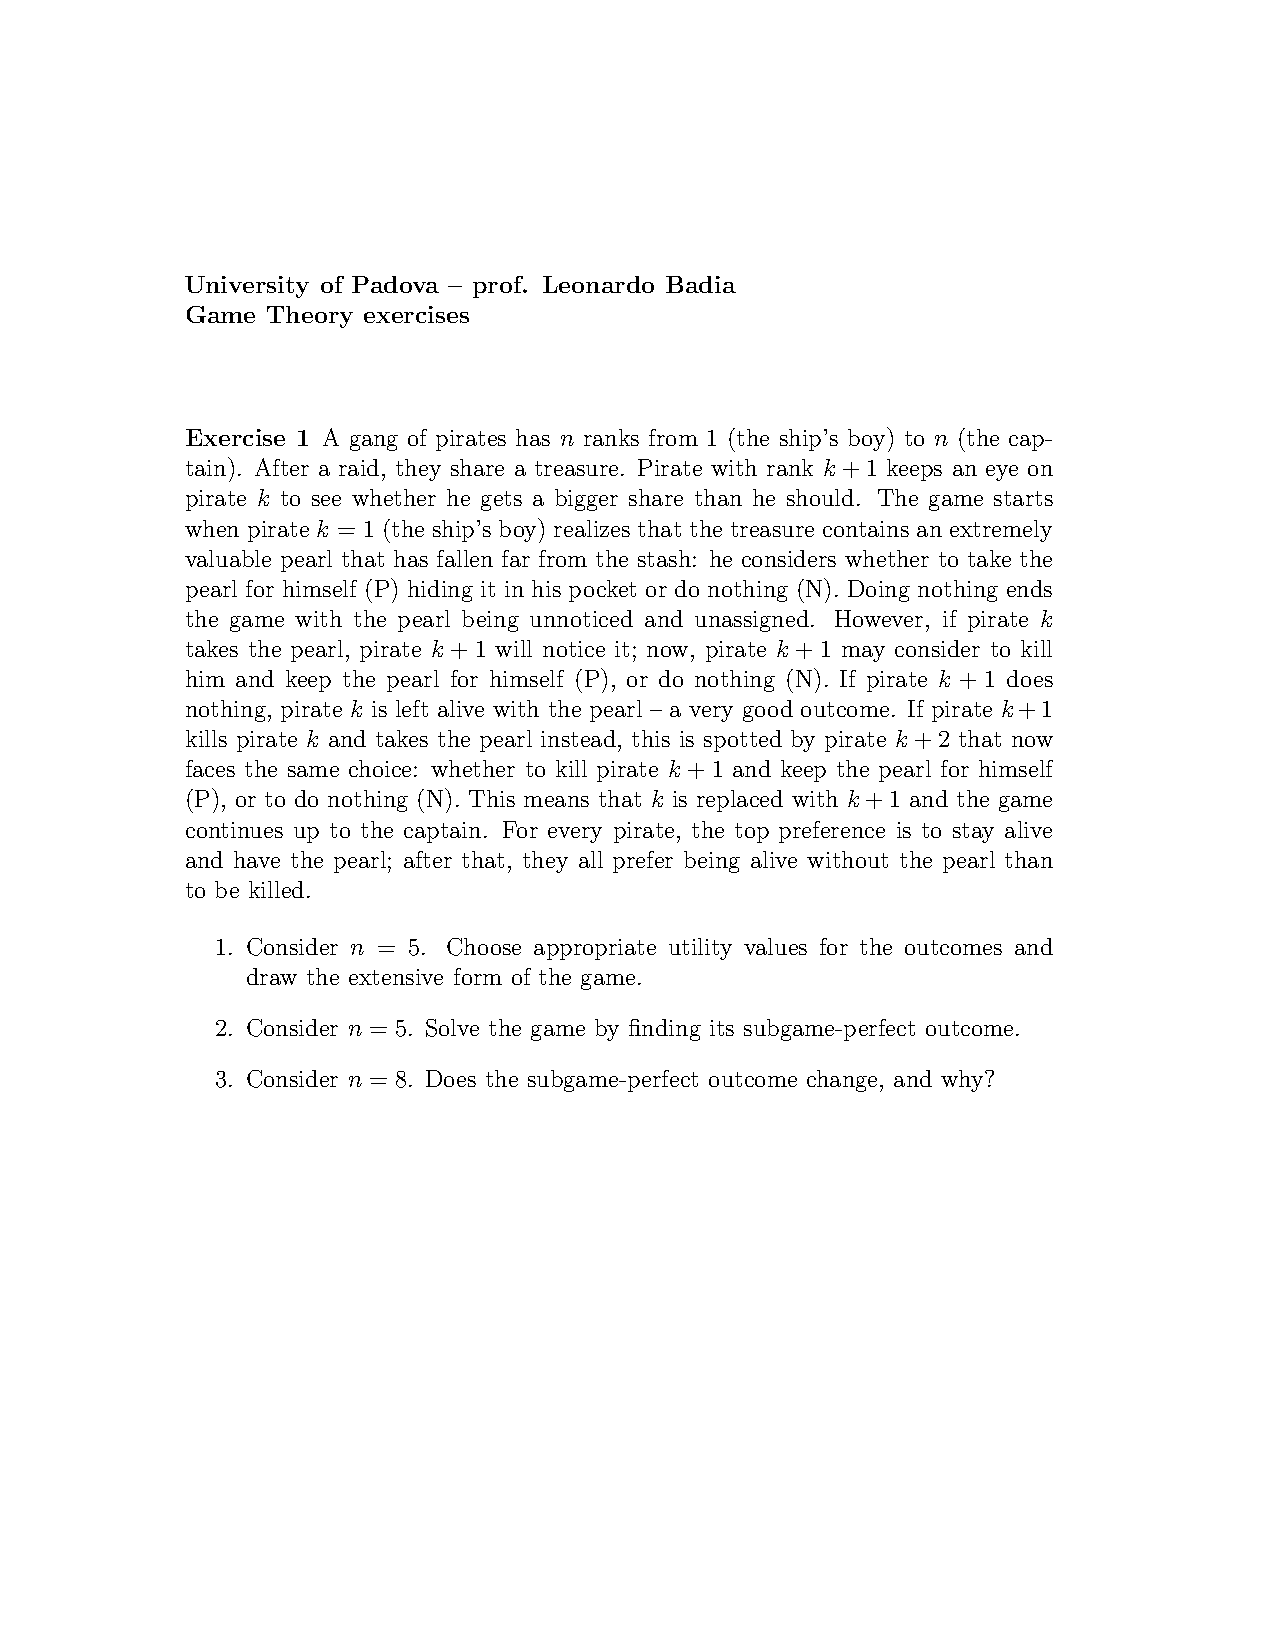
\includepdf[pages=-]{Appendix/Exercise3.pdf}
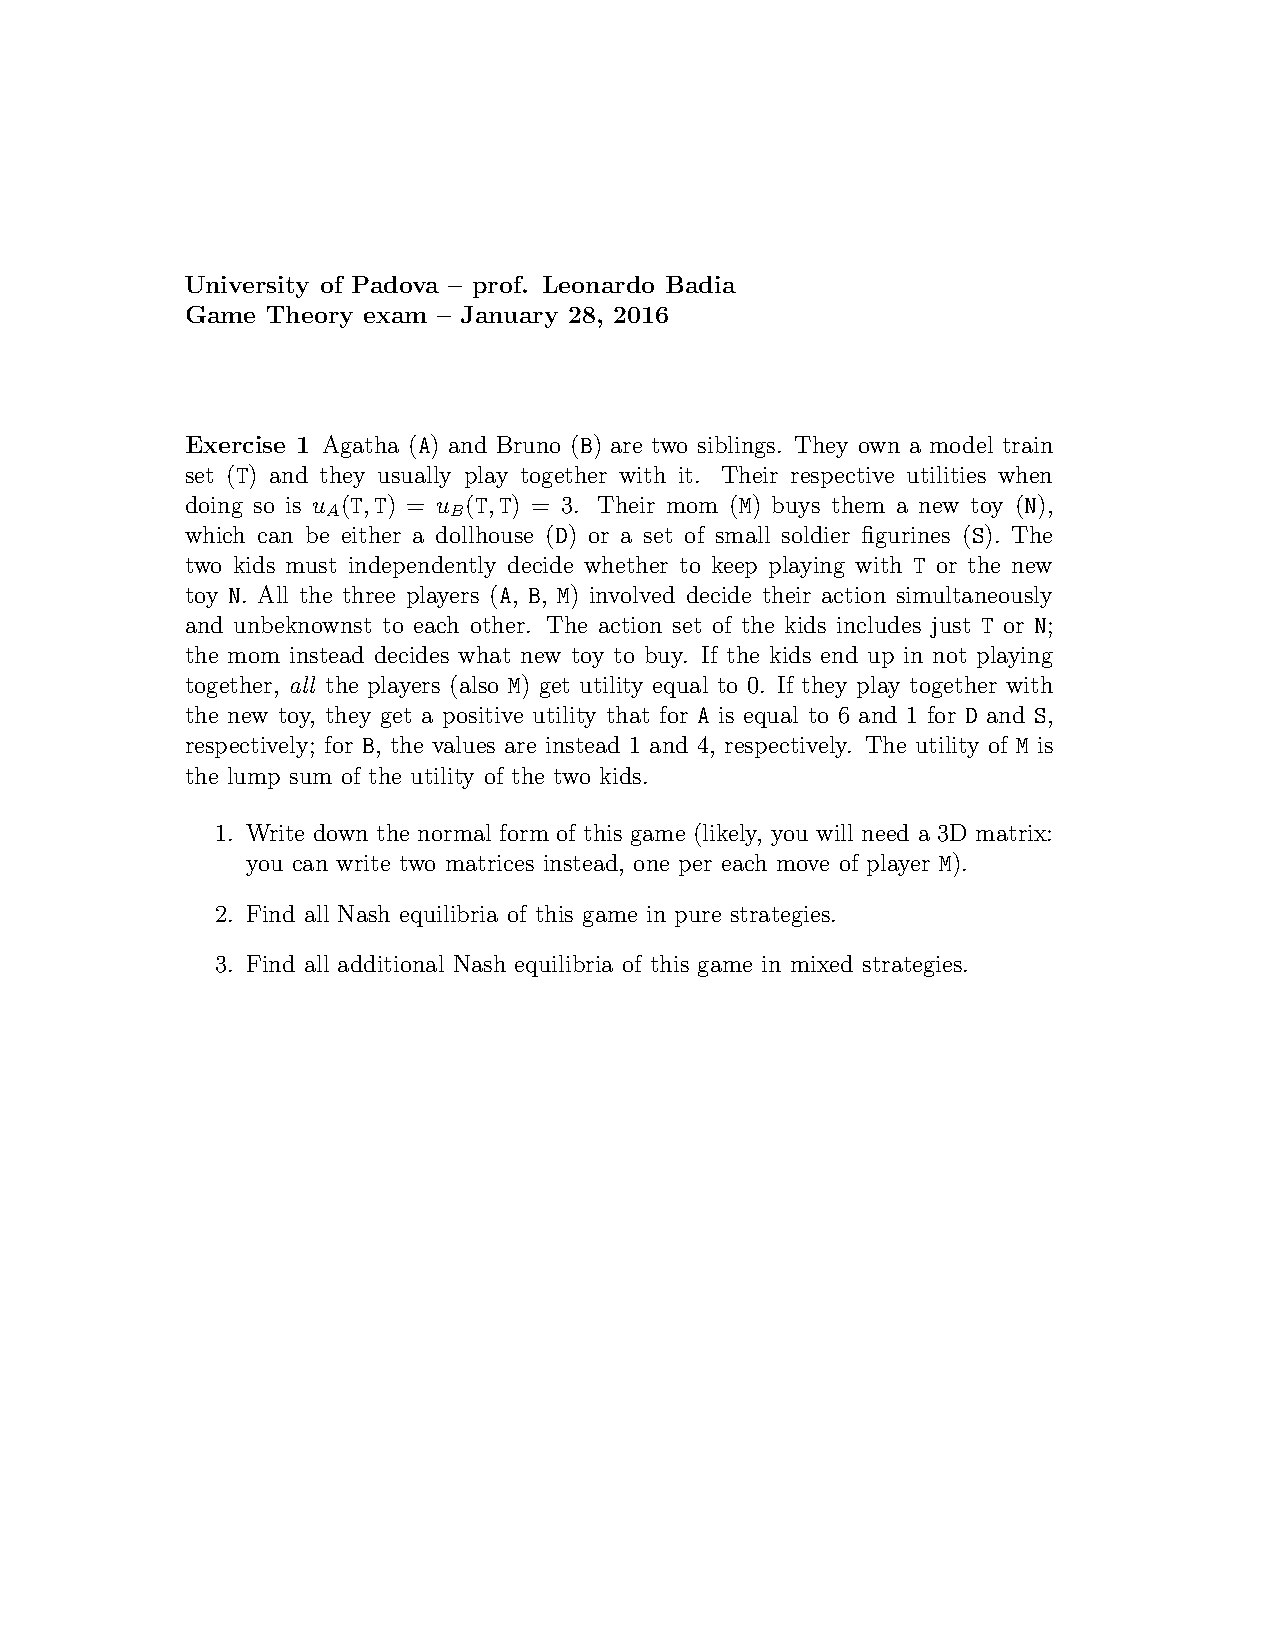
\includepdf[pages=-]{Appendix/Exam1.pdf}
\newpage
\section{Disclaimers}
For 2023-24 exam, professor said he will not ask for:
\begin{itemize}
    \item Dupolies
    \item Constitutions
    \item Potential games
\end{itemize}
\end{document}
